\documentclass[tikz, border=4pt]{standalone}
\usepackage{tikz}
\usepackage{chemfig}
\begin{document}
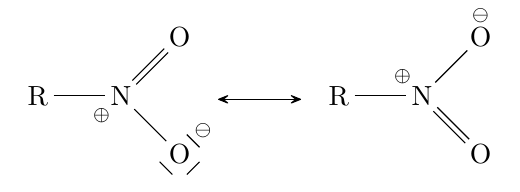
\begin{tikzpicture}[x=1cm, y=1cm]
  \node[anchor=north west, inner sep=0pt] at (0,0) {%
  \schemestart
    \chemfig{R-\charge{225:3pt=$\scriptstyle\oplus$}{N}([1]=[@{db}]@{atoo1}O)([7]-[@{sb}]@{atoo2}
    \charge{45=\|,-45=\|,-135=\|,45:5pt=$\scriptstyle\ominus$}{O})}
    \arrow(.mid east--.mid west){<->}
    \chemfig{R-\charge{135:3pt=$\scriptstyle\oplus$}{N}([1]-\charge{90:3pt=$\scriptstyle\ominus$}{O})([7]=O)}
  \schemestop
  \chemmove{
    \draw[shorten <=2pt, shorten >=2pt](db) ..controls +(120:5mm) and +(120:7mm)..(atoo1);
    \draw[shorten <=3pt, shorten >=2pt](atoo2) ..controls +(225:10mm) and +(225:10mm)..(sb);
  }%
  };
\end{tikzpicture}
\end{document}
